\documentclass[12pt]{amsart}
\usepackage{times}
\usepackage{courier}
\usepackage[margin=1in]{geometry}
\usepackage{amsmath,amsfonts,amssymb, amsthm}
\usepackage{bm}
\usepackage[ansinew]{inputenc}

\usepackage{graphicx}

\begin{document}
\title{\large CS 221 Project Final}
\author{Stuart Sy and Yushi Homma}
\date{December 11, 2015}
\maketitle
\section{\large Introduction of Task}
\label{def}
ESPN fantasy baseball is a common pastime for many Americans, which, coincidentally, defines a problem whose solution could potentially be predicted by artificial intelligence. The particular ESPN fantasy baseball game that we will analyze in this project is the ESPN Baseball Challenge. The basic task for these fantasy baseball participants is to predict which players will have successful games based on a standard scoring system and optimize the total score of their fantasy team under a budget. The fantasy teams consist of 9 players (one for each fielding position plus DH) and an entire pitching staff. This scoring system is provided by ESPN.com, which we define below in Section \ref{eval}.

\section{\large Literature Review}
Upon searching for literature on similar topics, I came across two related former Stanford CS 229 project papers. ``Predicting the Major League Baseball Season", written by R. Jia, C. Wong, and D. Zeng, regarded predicting wins and losses of teams in a particular season. Another that I came across, ``Applying Machine Learning to MLB Prediction \& Analysis" by Gregory Donaker, similarly tried to predict games to be wins or losses based on previous statistics. These two studies tried to predict the outcome of individual games, which is much more unpredictable than an entire season. This is because of the large amount of variance in games' outcomes, even among the same series. Our project differs in that it predicts the effectiveness of players across the entire season, so the effects of temporary slumps, good games, or bad games are factored into the season average.

\section{\large Input/Output}
\label{io}
The input into our system is the previous season's statistics. The system will then use this input to output the optimal team of 9 players of each position and a pitching staff with total budget of \$50 million.

\section{\large Dataset}
The dataset will include season statistics for every player in the MLB since 1871 matched with the scores of the corresponding players in the next season. We obtain this data from the baseball statistics archive accumulated by Sean Lahman in his collection of statistics found at http://www.seanlahman.com/baseball-archive/statistics/. The statistics for batters consist of the year played, their team, position, age, numbers of games, at-bats, runs, hits, 2B, 3B, home runs, runs batted in, stolen bases, attempts caught stealing, walks, and strikeouts. For pitchers, the dataset includes year played, team, age, salary, number of games, wins, games started, complete games, shutouts, saves, innings pitched (in outs), shits, earned runs, home runs, walks and strikeouts.

\section{\large Evaluation}
\label{eval}
The scoring system based on individual stats for the hitters and stats for the entire pitching staff of a team. The score for a single hitter is defined by the following formula:
\begin{equation}
\mathrm{Score_{hitter}} = \mathrm{R} + \mathrm{TB} + \mathrm{RBI} + \mathrm{BB} + \mathrm{SB},
\end{equation}
where 
$\mathrm{R}= (\mathrm{number\ of\ runs})$, $\mathrm{TB} = (\mathrm{total\ number\ of\ bases})$, $\mathrm{BB} = (\mathrm{number\ of\ walks})$, $\mathrm{RBI} = (\mathrm{number\ of\ runs\ batted\ in})$, and $\mathrm{SB} = (\mathrm{number\ of\ stolen\ bases})$. 
\vspace{.4cm}

The score for an entire pitching staff for a season is defined by:
\begin{equation}
3\cdot \mathrm{IP} - 3\cdot \mathrm{ER} - \mathrm{H} - \mathrm{BB} + \mathrm{K} + 5 \cdot \mathrm{W},
\end{equation}
where $\mathrm{IP}$ is the total number of innings piched, $\mathrm{ER}$ is the number of earned runs, $\mathrm{H}$ is the total number of hits that the pitching staff gave up, $\mathrm{BB} = (\mathrm{number\ of\ walks pitched})$, $\mathrm{K} = (\mathrm{number\ of\ strikeouts\ pitched})$, and $W = (\mathrm{number\ of\ wins})$.
\vspace{.4cm}

We will evaluate our system's predictions with the scores on the leaderboard of the ESPN Baseball Challenge listed for the past 4 years. These will be our test datasets.

\section{\large Infrastructure}
Using the pandas data science library, we extracted relevant parts of the CSV data and processed it into usable python objects. We separated the data by season because each season is one sample of data. We also determined what position each player is categorized as based on the metric given by ESPN.com (having played 20+ games at that position in the previous season). We also later matched up the playing statistics in Batting.csv and Pitching.csv with the calculated ages from Master.csv.

\section{\large Challenges and Approach}
This project poses two main challenges: to predict the scores of each player/pitching staff for the next season using the previous season's statistics and to find the maximum total team score within the constraints of the budget and player positions.
\vspace{.4cm}

Since the flow of a baseball game has natural breaks to it, and normally players act individually rather than performing in clusters, the sport lends itself to easy record-keeping and statistics. Ever since the explosion of fantasy sports, the analysis of player/team performance with statistics has become ever more popular/important. 
\vspace{.4cm}

As stated before, our task is to construct the best possible performing team (defined with a custom fantasy baseball score) under a budget constraint. To model this task, we want to model predicting the price/performance of individual players as a linear regression problem, and to model picking the optimal team as either a search or constraint satisfaction problem.
\vspace{.4cm}

One challenge that may be difficult to completely remedy is that our statistics only include season statistics instead of game-by-game statistics. This means that once we choose a team for a season, we have no additional information to change the members of the team during the season. However, in the ESPN Baseball Challenge, the fantasy baseball participants can change their rosters throughout the season, which could give them an advantage over our system due to fluctuations of players' performance throughout the season. This is why our oracle might not outperform the top participants of the ESPN Baseball Challenge, but it will be the best that we can aim toward with our algorithm.

\section{\large Baseline and Oracle}
We will perform our baseline and oracle on the year 2014. We defined our baseline to be just dividing the budget into equal parts to budget each individual position, and then obtaining the top salary player at each position that falls within the individual budget. The idea is that the teams would pay their more valuable players with higher salaries, so their salary is their projection of how the player will perform the next year.
\vspace{.4cm}

We used 3/10 of the budget on the pitching staff because that is roughly how much MLB teams pay their pitchers. This leaves 3.9 million for each hitter and 15 million for the pitching staff. This resulted in a score of 3712. We defined our oracle to the best team for 2014, knowing the 2014 actual scores beforehand. We just used our improved CSP algorithm to calculate this value, which was 6151. Thus, there is room for much improvement from the baseline to the oracle.

\section{\large Machine Learning}
The primary portion of our task was to predict the each year's scores of each player using the previous year's statistics for that player. There are a number of ways that we could have carried out the task, but we decided on testing multiple linear regression, logistic regression and support vector regression. We found that the linear regression performed the best in all cases (explained in Section \ref{error}), so the rest of this section will focus on our choice of linear regression. An advantage of using linear regression is that there is not much need to know much about how each variable factors into the prediction. Thus, the work lies in finding good features for the predictor to work with.
\vspace{.4cm}

The features we used clearly needed to include all of the factors taken into account in calculating the score. Thus, for batters, we included the number of runs, hits, doubles, triples, home runs, runs batted in, walks, and stolen bases. For pitchers, we included the number of innings pitched, earned runs, hits, walks, strikeouts and wins. However, we had many more stats at our disposal. We only included the stats that we thought would have a direct effect on the score next year. This included much of the stats regarding their performance in games, and very little of the biographical information like college and hometown. 
\vspace{.4cm}

These other features that we believed to be relevant for batters are: weight, height, strikeouts, times caught stealing, age and salary. We believed that weight, height and age could somehow help predict the longevity of the players' skills and maybe predict the trends of their growth and slumps. We also believed that their salary could help with other unquantifiable factors like star potential or popularity that could factor into their score for the next year. The strikeouts and times caught stealing are negatives for batters that could indicate a potential for slumps; for example, if a fast player is getting caught stealing more often, it could indicate that he will not steal bases as much the next year because his running skills are deteriorating. 
\vspace{.4cm}

For pitchers we had games played, innings pitched (measured in outs), home runs, the opposing batters' batting average, saves, runs, shut outs, earned runs average, weight, height, year and salary. We included weight, height, and salary for the same reasons as the batters. The rest of the game statistics are pretty clear in their potential effects on the next year's score. 
\vspace{.4cm}

For the algorithm, we treated the batters and the pitchers as distinct datasets. We used KFold from sklearn.cross\_validation package to cross validate our data in order to avoid overfitting to the training data. We used LinearRegression from sklearn.linear\_model package to train a predictor of the scores for each player. We used these predicted scores in the CSP part that is explained in the following section.
\section{\large Constraint Satisfaction Problem}
The constraint satisfaction problem involved picking one player from each position and a pitching staff to maximize score with the given budget of \$50 million. This part proved to be quite a challenge because the amount of computing involved in solving the CSP is enormous to find all the budget-satisfying teams of 9 players and a pitching staff. Thus, we were met with no success when we first tried just implementing the CSP algorithm from class.
\vspace{.4cm}

For this first attempt, we first had to sum the salaries and predicted scores of the pitching staff for each team and store them as one entity. Then, we modeled the problem with each position (including pitching staff) as a variable with the domains being all the players with that position. The players were represented by a tuple of their ID, score, salary and position. Then, we only had one factor: the sum of the salaries of each position had to be at most \$50 million.
\vspace{.4cm}

To actually implement the algorithm, we implemented the get\_sum\_variable function of the CSP homework. To solve the constraint satisfaction problem, we just used the python-constraint package to input the model and it returned all the possible solutions. Then we just took the solution with the maximum score because we know that all these solutions satisfied the constraint.
\vspace{.4cm}

However, this algorithm did not terminate even after 3 hours of computation. Thus, we deviated from the initial approach and used the fact that we only needed the best team, not all possible teams, to simplify the computation. 
\vspace{.4cm}

First, for each position, we deleted all players who had higher salaries but lower scores/predicted scores than someone else of the same position. These players could never be on a best team because the other player could be switched in to make a better team score. This process greatly diminished the number of players the algorithm had to consider.
\vspace{.4cm}

Then, we sorted the players of each position in order of increasing salary. Then, we performed a simple CSP algorithm to find teams that satisfied the budget by just by successively adding each position to partial teams and throwing out teams that already went over budget. We did this for every position besides the pitching staff. 
\vspace{.4cm}

For the pitching staff, we just tried adding each staff to a team in decreasing salary order until the team is not over budget and checked if that full team was better than the best team found before. If it was, it became the new best team and we moved on to the next partial team. This optimization also does not affect the result because each pitching staff with a lower salary than the first one that satisfied the budget has a lower score as well. 
\vspace{.4cm}

The best team that remained at the conclusion of this algorithm was returned with its final total salary, its total score, and its list of players. The improved CSP algorithm proved to be much faster and could find the best team among a league of approximately 300 \"players\" (Pitching staffs considered as one player and rookies neglected) in about 5 minutes.

\section{\large Initial Experimental Results}
We ran our algorithm on the 2010 data predicting the 2011 scores. We found out that the linear regression had an average absolute difference from the actual scores of 78.55 for pitchers. We found that it had an average absolute difference of 87.36 for batters. This shows that the choice of features may not have been the best or that the trends of players may not be linear as there is still quite a bit of room for improvement. When we did this initial experiment, we did not have a working CSP algorithm, so we could not compare with the baseline and oracle.

\section{\large Improvements on Feature Choice}
Upon seeing the room for improvement on the linear regression portion, we realized the absence of any obvious time-sensitive factors. These are important because they would help to predict changes in a player's fantasy score from year to year. Thus, by suggestion of Arjun Puranik, we decided to add both age and difference of the previous two years' scores as features. However, since some players did not have two previous years' scores, we gave such players the median score of that year to calculate the difference. 
\vspace{.4cm}

Yet, for some reason, this ended up decreasing the score of our calculated best team, so we checked the weights that resulted in the linear regression. This analysis revealed multiple counterintuitive weights:
\begin{itemize}
	\item The newly added delta\_score weight was negative, implying that players who improved the past year would not improve the next year. \\
	\item Caught stealing had a positive weight, which would imply that getting out while stealing is a positive factor. \\
	\item Doubles had negative weight, even though it is a positive influence on score.\\
	\item Games played for pitchers was negative weight, even though the more games means a better score.
\end{itemize}
\vspace{.4cm}

With these factors with counterintuitive weights, we removed them from the prediction factors considered in the linear regression. We were met with decent success, adding anywhere from 50 to 150 points to the calculated best teams' total scores for each year.
\section{\large Analysis of Results} \label{error}
Our algorithm's slowest part is the CSP because the time complexity is $O(\#\ \mathrm{teams}\ \mathrm{searched})$. The number of possible teams is the product of the number of players at each position. Thus, the time complexity of our CSP algorithm, and total time complexity, is $O((n/10)^10) = O(n^10)$. The memory used is also the same because the algorithm had to store each of these teams with their player names, salary and score.
\vspace{.4cm}

As mentioned earlier, one of the choices that we made for the algorithm was which machine learning algorithm to use for predicting the score of each player. The graph below illustrates the scores of each of the algorithms considered in comparison with the oracle. Linear regression was the clear winner, with logistic regression and support vector regression scoring an average of over 1000 below linear regression.
\vspace{.4cm}
\begin{center}
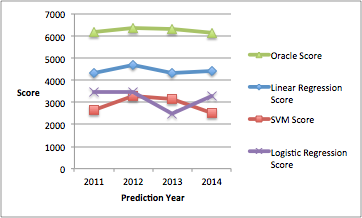
\includegraphics[scale=0.9]{graphimage.png}
\end{center}

Below is a table showing the results of our final algorithm in calculating the best team score possible for the years 2011-2014. 
\vspace{.4cm}
\begin{center}
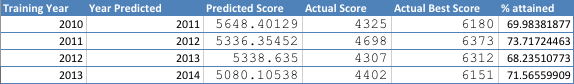
\includegraphics[scale=0.8]{table.png}
\end{center}
\vspace{.4cm}

This table shows that our predicted scores from linear regression on the previous year's statistics are much higher than the actual scores calculated from the current year's statistics. This demonstrates the limitation of our algorithm in predicting the effectiveness of a player using his previous statistics.

\section{\large Conclusions and Future Work}
We found that even predicting a player's season rather than just one game is still variable to unseen factors. Furthermore, it is difficult to determine when a player will peak, which made the time-dependent factors less effective. Compared to our baseline in 2014, our algorithm performed approximately 700 points above, which is a significant amount. However, seeing that our algorithm still fell well below the oracle every year, there is still quite a bit of room for improvement. Nevertheless, this project showed that it is possible to improve on the teams' predictions of the value of their players by using machine learning on just the previous year's statistics.
\vspace{.4cm}

One possible avenue for improvement would be to scrape and utilize game-by-game statistics to calculate more time-sensitive variables other than just age (delta\_score proved to be ineffective). Another way we could improve the predictions is by using statistics from multiple years before the prediction year instead of just one. The idea is that we could capture trends from year to year for each player; however, the problem is that the more previous years we use, the less players we have that actually played all of those years. These possible areas for future work could improve our algorithm closer to the oracle due to the more accurate projection of player trend.
\end{document}